\section{Introduction}
This chapter presents the CPIM library extension. Sections \ref{sec:cpim-architecture} and \ref{sec:kundera-integration} describe the previous state of the NoSQL service in the CPIM, the changes made to integrate Kundera as unique persistence provider and the problems faced during the process.

\noindent From section \ref{sec:hegira} up to section \ref{sec:data-interoperability} are described the various parts we developed to support \textit{Hegira}, an interoperable data migration sand synchronization system for NoSQL databases \cite{paper:modaclouds-deliverable}, describing the supported features and the design choices that have been put in place. 

\section{CPIM architecture}
\label{sec:cpim-architecture}
In order to be able to expose a common interface for the multiple services supported by the library, CPIM adopts heavily the factory and singleton patterns.

\noindent The main access point of the library is the \texttt{MF} (Manager Factory) class, a singleton object which is responsible of reading the configuration files and exposing a set of methods that will build instances for the service factories.
The initialization is done through a first call to the \texttt{MF.getFactory()} method, which reads the configuration files and build an instance of the \texttt{CloudMetadata} class; this class will be referenced by all the other services and it contains all the information stored in the configuration files.
 
\newparagraph The CPIM library is organized in several packages, each of which is responsible of a particular service.
\noindent Each service exposes a factory class which is invoked through the \texttt{MF} factory; the service factory maintains a singleton instance of the provider-specific service implementation which is built, at the first call, based on the configuration available inside the singleton instance of \texttt{CloudMetadata}.
The result of this process is that with the same method call, based on the configuration file, can be instantiated a different service implementation.

\subsection{NoSQL service}
The architecture of the NoSQL service before this work has been reported in figure \ref{fig:cpim-nosql}.

\begin{figure}[tbh]
  \centering
  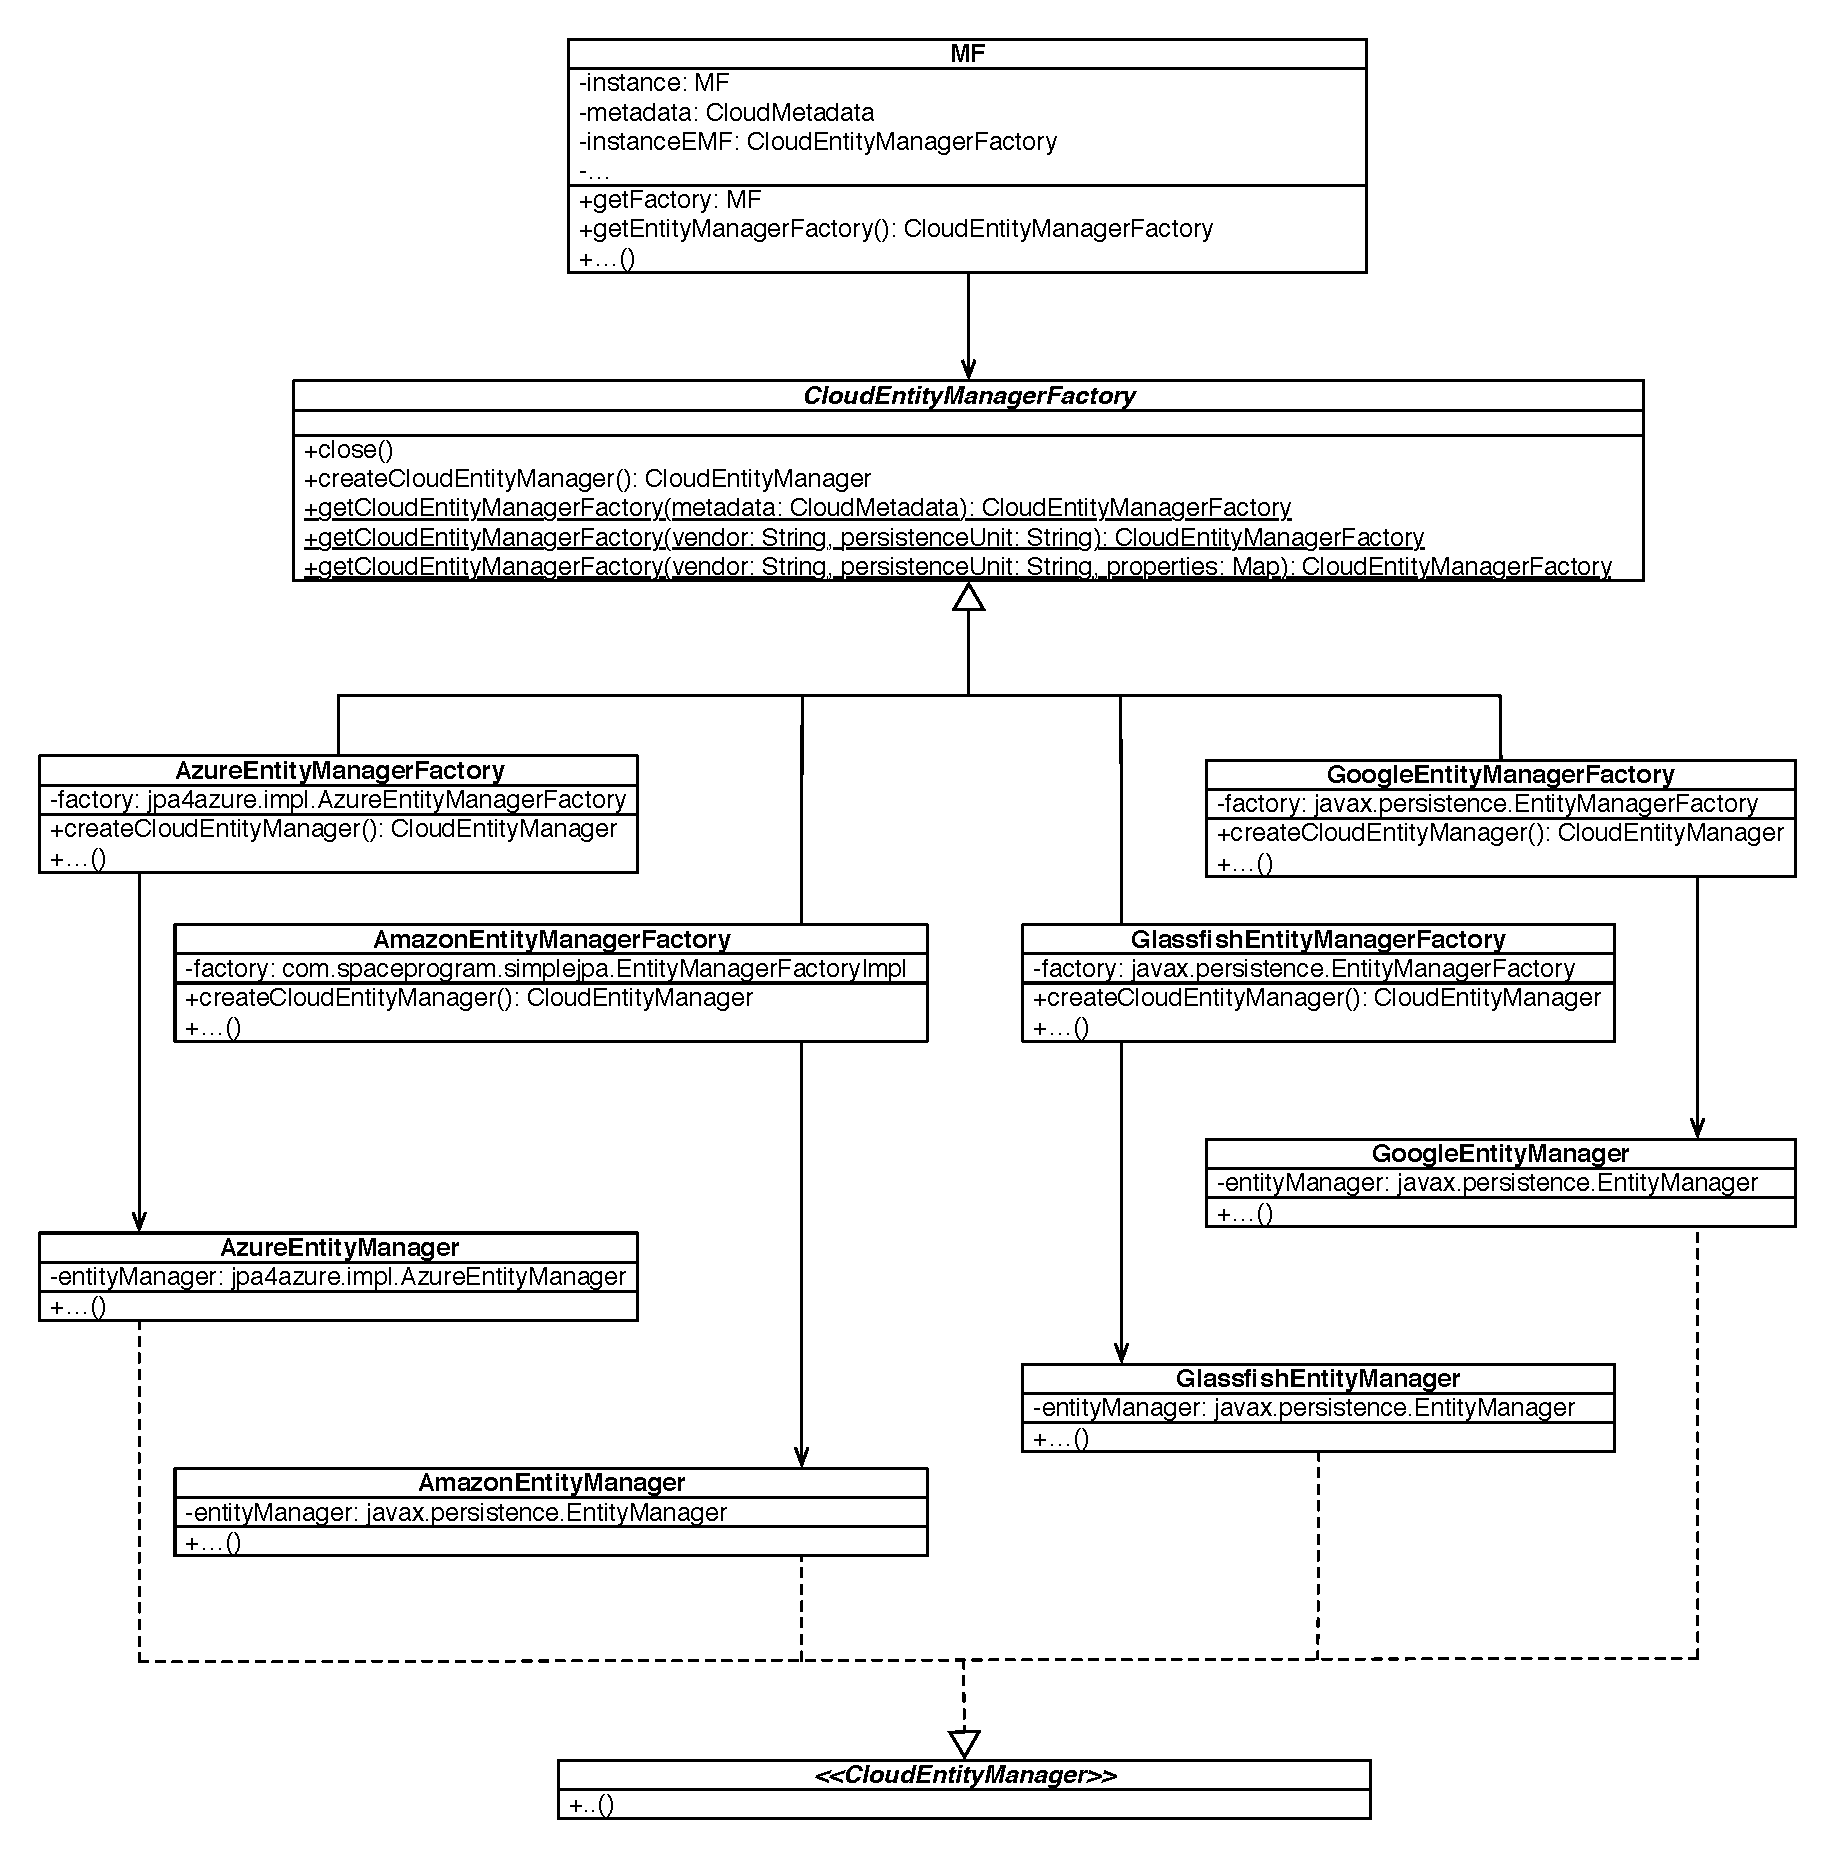
\includegraphics[width=14cm]{images/cpim_nosql_old}
  \caption{NoSQL service architecture}
  \label{fig:cpim-nosql}
\end{figure}

\noindent To use the service, the first step is to instantiate a \texttt{CloudEntityManagerFactory} and, depending on the configuration file, this factory instantiates the vendor specific factory. For example, in case Google is chosen as vendor, the instantiated factory will be \texttt{GoogleEntityManagerFactory}. 
Each provider-specific \texttt{EntityManagerFactory} is responsible of instantiating an \texttt{EntityManager} which is the gateway to the underlying database. All vendor-specific \texttt{EntityManager}(s) implement the common \texttt{CloudEntityManager} interface to achieve uniformity in methods and behavior.
The various implementation of the \texttt{CloudEntityManager} delegates every method call to the vendor-specific persistence provider. 

\newparagraph The JPA is not a default language for NoSQL but, due to its wide usage among Java developers, several JPA implementations have been built for various NoSQL databases (both developed by the vendor of the NoSQL storage or by the community).
This means that to support the NoSQL service through the JPA interface, an implementation of the JPA interface must be found or developed \textit{ad hoc}. For this reason there were three different persistence providers in the CPIM library, one for each cloud provider:
\begin{itemize}
\item for \textit{Google Datastore} an official JPA implementation (available inside the SDK) was used;
\item for \textit{Amazon SimpleDB} it used \textbf{SimpleJPA}, a third-party implementation of the JPA interface;
\item for \textit{Azure Tables} it used \textbf{jpa4azure}, a third-party implementation of the JPA interface.
\end{itemize}

\noindent There are a couple of things to notice: Amazon SimpleDB has been deprecated in favor of DynamoDB and \textit{jpa4azure} is not being maintained anymore, therefore the CPIM library needs to be updated in order to get rid of those outdated software.

\section{Kundera integration}
\label{sec:kundera-integration}
To solve these problems and reduce the number of software on which the CPIM relies to provide the NoSQL service, the proposed solution is to modify the current CPIM architecture with a unique persistence provider that has been identified in Kundera.

\newparagraph The renewed architecture is resumed in figure \ref{fig:cpim-kundera} in which the benefit of having a single JPA provider are clearly visible, the architecture is slightly less articulated and no check on the selected underlying technology is needed since this is handled by Kundera, while reading the \textit{persistence.xml} file, in which the user defines the databases he is interested in.
Another benefit of this architecture is that the choice of the NoSQL technology is not bound to the vendor specified in the CPIM configuration file anymore, in fact, it is possible, by configuring the \textit{persistence.xml}, to deploy the application in one of the supported PaaS providers and choose to persist the data in a NoSQL database of another provider. Moreover it is possible to exploit the Kundera polyglot persistency to persist part of the data in a database and another part in another one, defining the persistence units accordingly.

\begin{figure}[tbh]
  \centering
  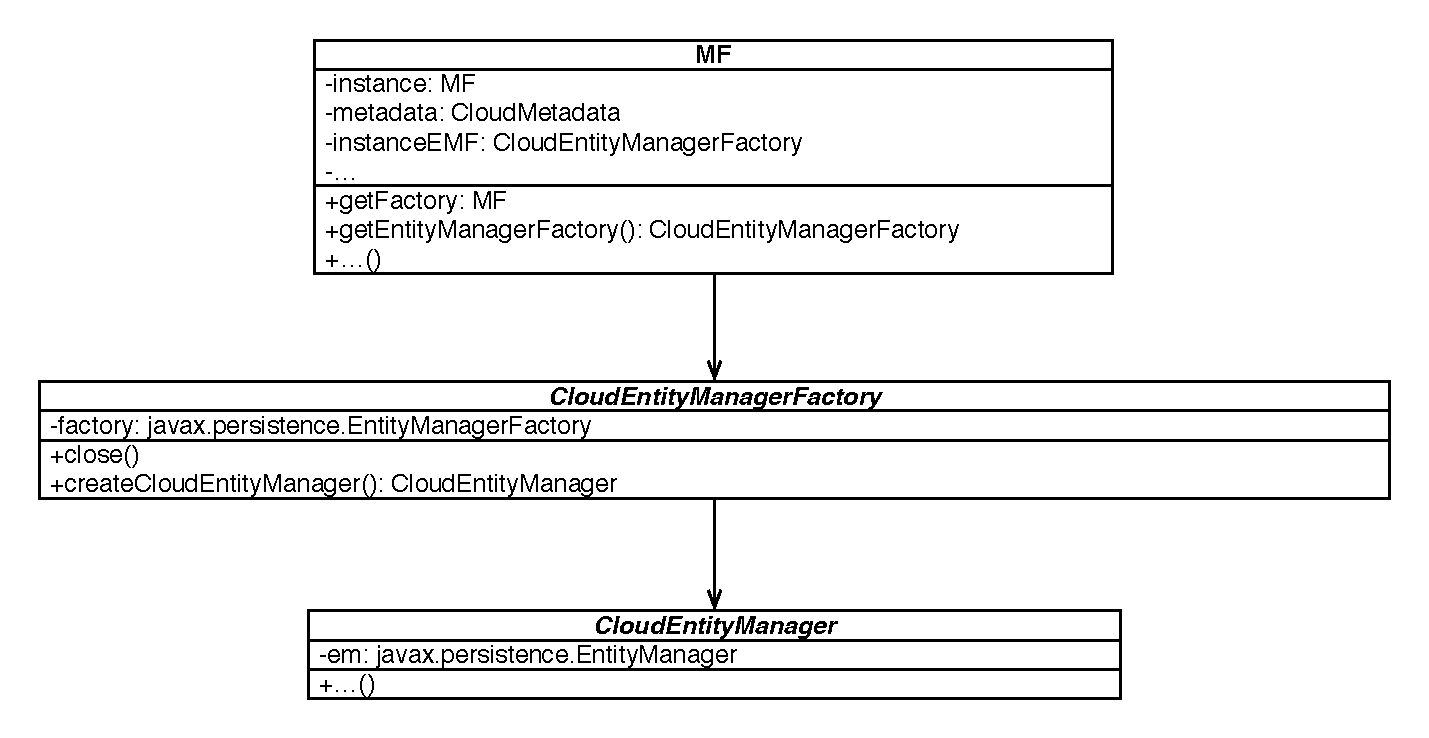
\includegraphics[width=14cm]{images/cpim_nosql_kundera}
  \caption{The modified NoSQL service architecture}
  \label{fig:cpim-kundera}
\end{figure}

\noindent The actual implementation is completely provider agnostic in the sense that actually Kundera is not required as dependency and in fact it is not listed as a dependency for the CPIM. At run-time, when a Kundera client will be listed among the dependencies of the user application, as well as the CPIM library, the persistence provider dependency will be satisfied.

\noindent This provider agnostic implementation is due to the fact that the \texttt{CloudEntityManagerFactory} and the \texttt{CloudEntityManager} respectively implement the JPA interfaces \texttt{EntityManagerFactory}  and \texttt{EntityManager}.
The actual call to the run-time provider is made within the \texttt{CloudEntityManager} that, on construction, instantiate an instances of the provider \texttt{EntityManager} and uses that reference to delegate every method execution to it.

\noindent This can seem an over-designed architecture, but it turns out to be extremely necessary in order to provide a transparent interaction with the migration system, as it will explained later on in this chapter.

\subsection{Problems encountered}
\label{sec:cpim-problems}
Kundera provides an uniform access through the JPA interface, independently from the NoSQL provider which is being used. The desired target database is defined in the \textit{persistence.xml} file through the \texttt{kundera.client.lookup.class} property. For this reason all the old libraries that provide a JPA implementation for a specific vendor can be removed from the CPIM. 
This tentative of cleaning the dependency of the CPIM caused two main problems:
\begin{enumerate}
\item \textit{jpa4azure} turns out to be used also for Queue and Blob service of Windows Azure;
\item Kundera seems to have problems when multiple persistence providers are found in the classpath and currently no way to force the selection of Kundera as persistence provider has been found (besides specifying it in the \textit{persistence.xml} file).
\end{enumerate} 

\noindent To solve the first problem, the code of the extended version of \textit{jpa4azure} has been inspected. We found that the library was previously extended to support some missing functionalities of the JPA interface and contained two main packages:
\begin{itemize}
\item \texttt{jpa4azure}, which contained the code that implements the JPA interface;
\item \texttt{com.windowsazure.samples}, which contains the code to ease the communication with the Azure services.
\end{itemize}
The \texttt{jpa4azure} package has been removed and the library rebuilt since the other package is the one used in the Blob and Queue service. Its possible to completely remove \texttt{jpa4azure} but is necessary to rewrite also the CPIM Blob storage service for Azure using the API provided by the Azure SDK.

\newparagraph Removing the \texttt{jpa4azure} library caused unexpected errors in CPIM in the code of the Queue service. After some investigations, turns out that, when \textit{jpa4azure} was extended, the class \texttt{AzureQueueManagerFactory} were introduced.
The problem was that \texttt{AzureQueueManagerFactory} make use of the JPA interface to communicate with the Queue service of Azure and thus by removing the support to the JPA interface we have lost the support for Azure Queue service.
A solution to this would be to rewrite the CPIM Queue service for Azure, using the API provided by the Azure SDK.

\section{Hegira integration}
\label{sec:hegira}
To support data synchronization and migration, the NoSQL service was further modified to integrate \textit{Hegira} \cite{thesis:marco}. We have defined the interaction mechanism required to make the CPIM library able to communicate with \textit{Hegira} and summarized it in the high level schema reported in figure \ref{fig:high-level-interaction}.

\begin{figure}[tbh]
  \centering
  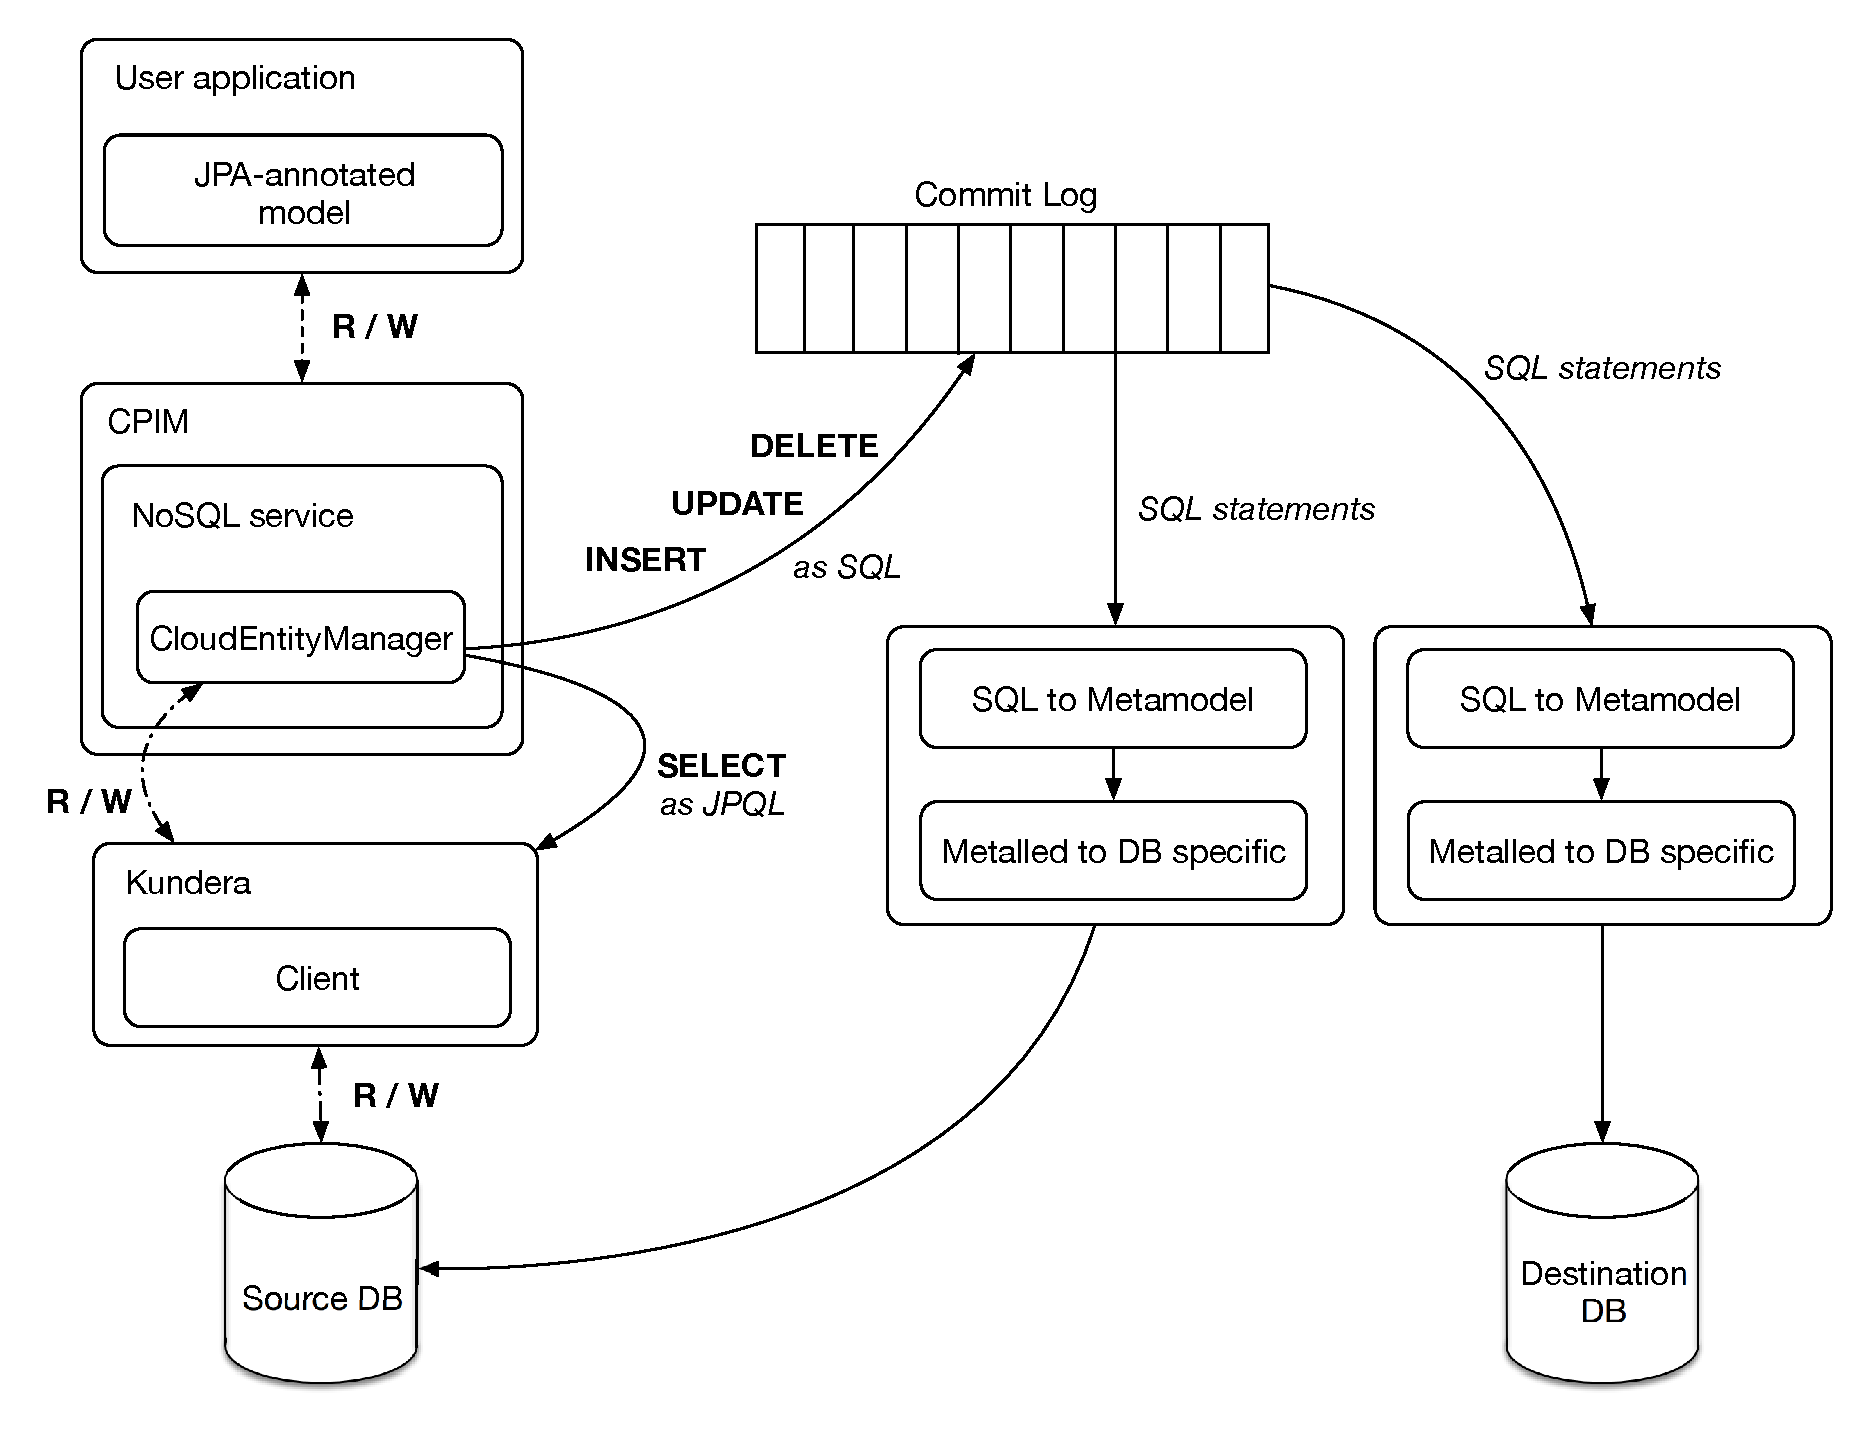
\includegraphics[width=11cm]{images/high_level_interaction}
  \caption{High level schema of interaction}
  \label{fig:high-level-interaction}
\end{figure} 

\newparagraph  The user interacts with the NoSQL service of the CPIM library by using the JPA interface by expressing operations on the data though the \texttt{EntityManager}, for CRUD operations, or through JPQL queries. 

\noindent The normal operations flow is reported in the schema of figure \ref{fig:high-level-interaction} with \textbf{dashed} lines. In this scenario, user operations are delegated by the CPIM library to Kundera that, ultimately, interacts with the underlying database using the appropriated client.

\noindent In the same figure, with \textbf{filled} lines, is reported the operation flow that needs to be followed when a migration is in process; user operation are intercepted and sent to the commit log of \textit{Hegira} from which are then pulled and written asynchronously on both the destination database and the source database.
 
\noindent The CPIM library needs to connect to the migration system in order to understand when a migration is in progress to be able to choose the right destination of the user operations. Data manipulation operation, such as UPDATE and DELETE queries, and CRUD operations, are intercepted, translated in an equivalent SQL operation and sent to the commit log of \textit{Hegira}.
The process is summarized in figure \ref{fig:flow-chart} and described in detail in section \ref{sec:intercept-user-operations}.

\begin{figure}[tbh]
  \centering
  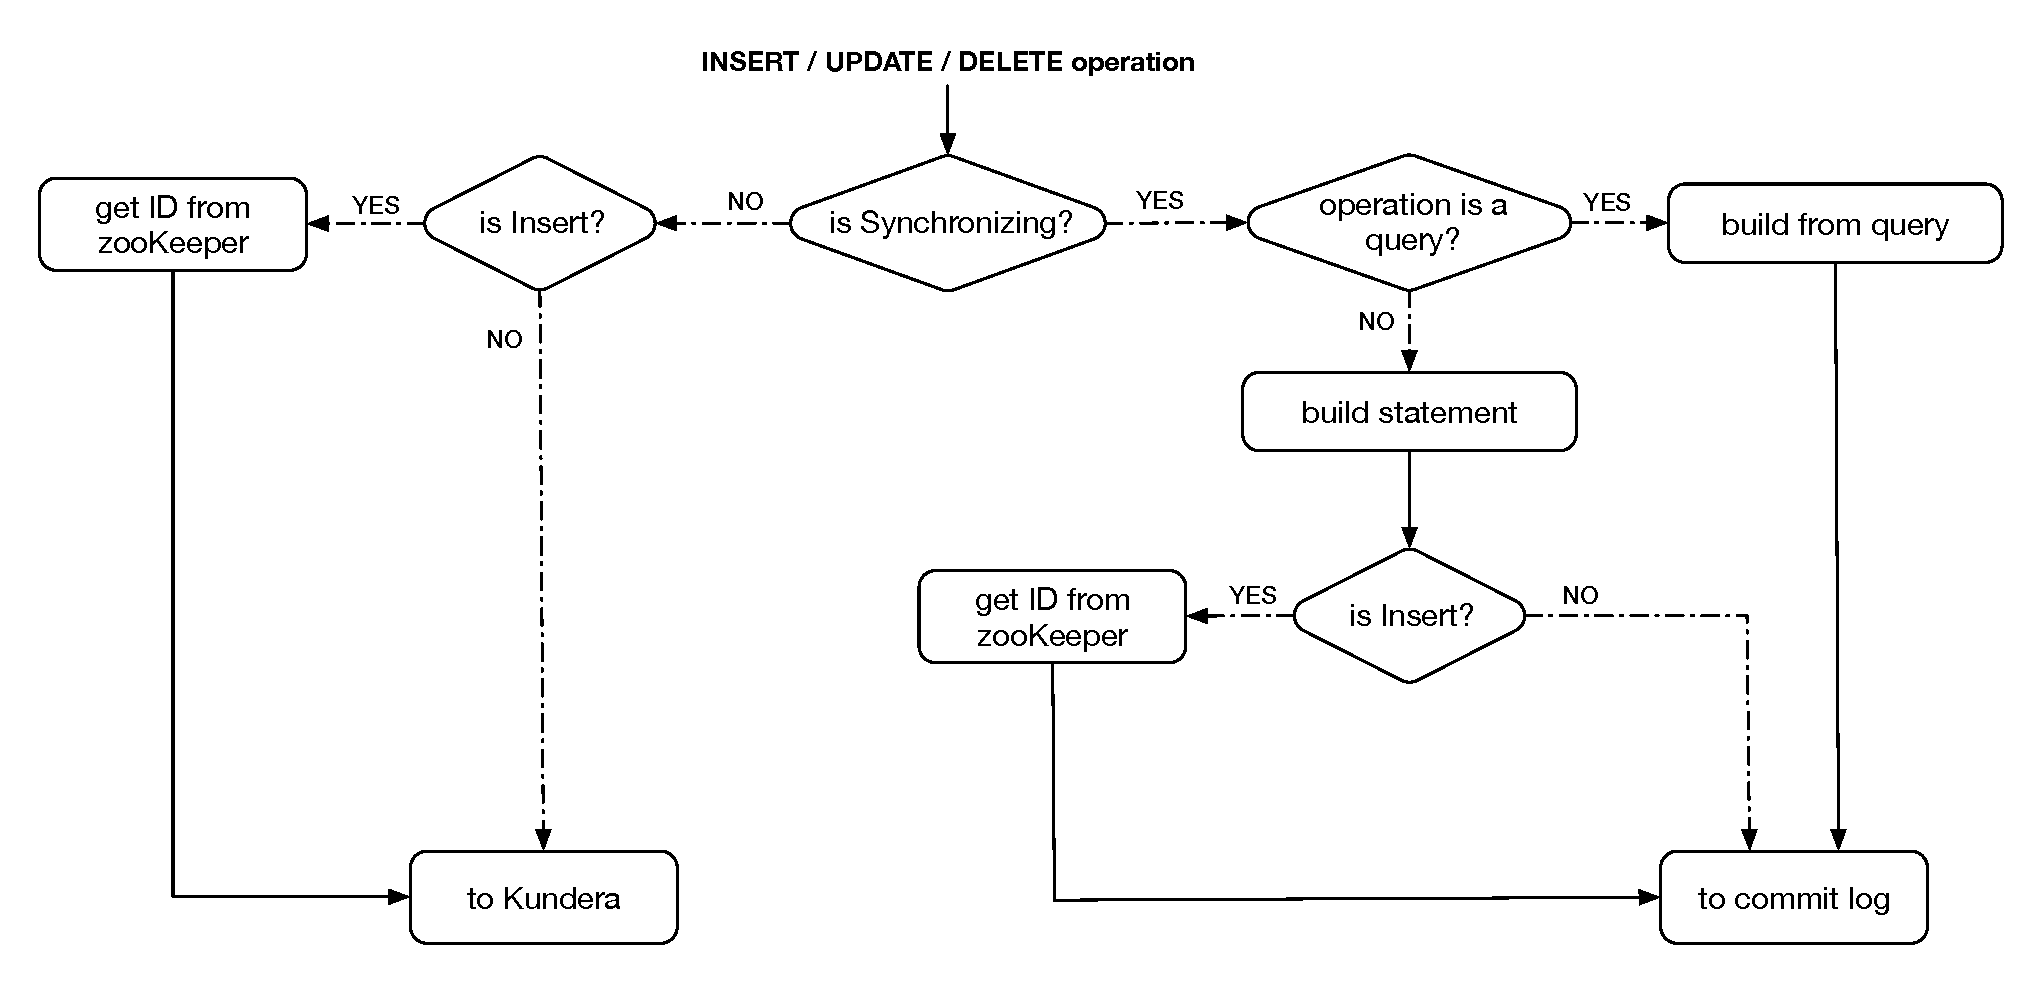
\includegraphics[width=12cm]{images/flow_chart}
  \caption{Interaction flow chart}
  \label{fig:flow-chart}
\end{figure} 

\noindent While data manipulation operations are intercepted, read operations, such as SELECT queries, are ignored and thus also during a migration, they are issued on the underlying databases by delegating them to Kundera.

\subsection{Migration Manager}
Interaction with the migration system is handled primarily by the \texttt{MigrationManager} class which follows a state pattern represented in the class diagram \ref{fig:migration-class-diagram}. 
 
\begin{figure}[tbh]
  \centering
  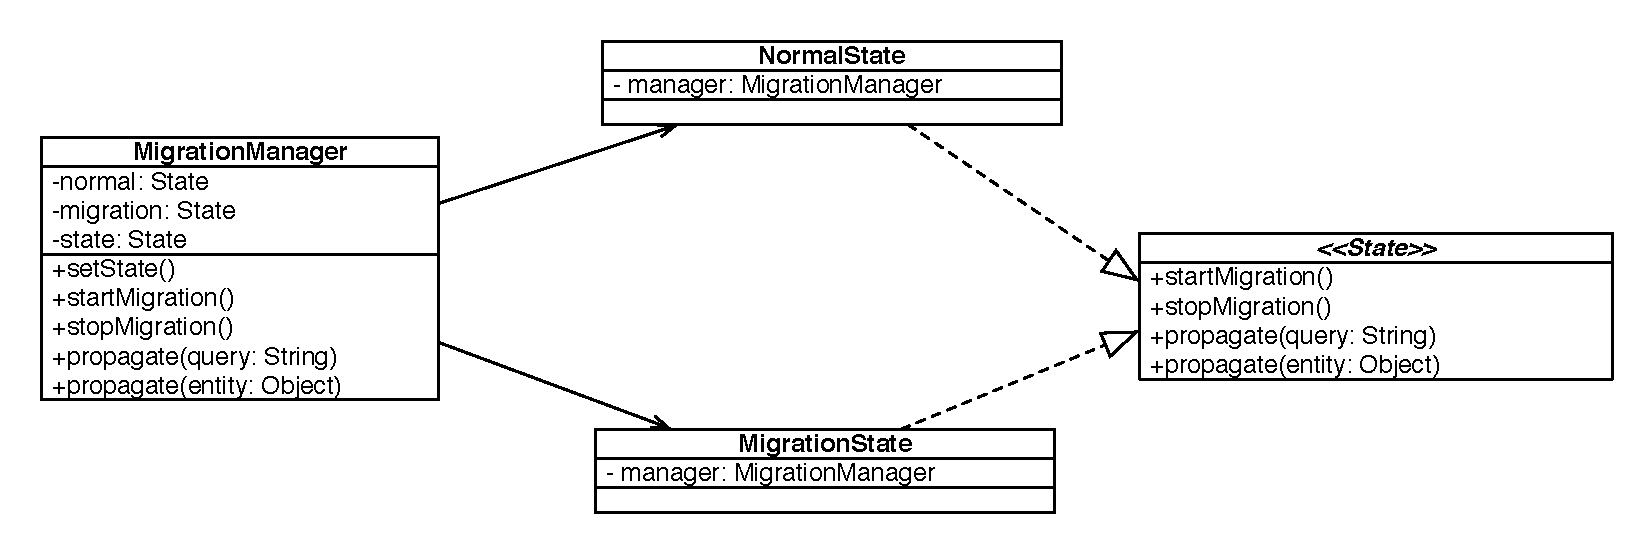
\includegraphics[width=14cm]{images/migration_class_diagram}
  \caption{\texttt{MigrationManager} class diagram}
  \label{fig:migration-class-diagram}
\end{figure} 

\noindent The pattern allows to the \texttt{MigrationManager} to delegate the method execution to the current state, the state diagram is the one represented in figure \ref{fig:migration-fsa} and is composed by two states \texttt{Migration} and \texttt{Normal} that encapsulate the required behavior.
    
\begin{figure}[tbh]
  \centering
  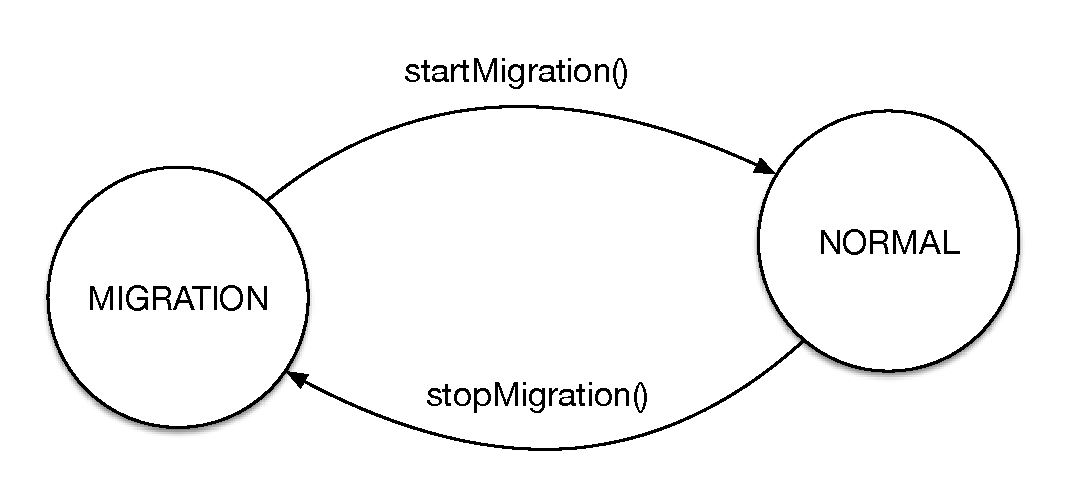
\includegraphics[width=6cm]{images/migration_fsa}
  \caption{\texttt{MigrationManager} states}
  \label{fig:migration-fsa}
\end{figure} 

\section{Intercept user operations}
\label{sec:intercept-user-operations}
The first operation that needs to be analyzed is whether it is possible to intercept user operations in a way that is completely transparent to the user.
The operations that we want to intercept are the insert, update and delete operations, in that, they are the operations that alter data and, thus, are the ones that the synchronization system needs to process.

\subsection{Intercepting CRUD operations}
CRUD operations are handled by the \texttt{EntityManager}, three are the methods that need to be intercepted:
\begin{itemize}
\item \texttt{EntityManager.persist(Object entity)} for insert operations;
\item \texttt{EntityManager.merge(Object entity)} for update operations;
\item \texttt{EntityManager.remove(Object entity)} for delete operations.
\end{itemize}
\noindent The user does not invoke methods directly on the provider entity manager, but he interacts with the persistence provider, through the \texttt{CloudEntityManager} class. In the standard implementation (i.e. without the support for the migration system) the \texttt{CloudEntityManager}, delegates every method call to the provider entity manager; hence, in order to integrate the  migration and synchronization logic, the methods mentioned above should contain the application of logic shown in the snippet of code \ref{code:isMigrating}, which takes as an example, the update operation.

\begin{lstlisting}[language=Java, caption=Integrate migration logic, label=code:isMigrating]
public <T> T merge(T entity) {
    if (MigrationManager.isMigrating()) {
        MigrationManager.propagate(entity, OperationType.UPDATE);
        return entity;
    } else {
        return delegate.merge(entity);
    }
}
\end{lstlisting}

\noindent In case of data migration, the provider is bypassed and a call to the \texttt{propagate} method is visible. The call accepts two arguments: the entity to be converted to a SQL statement and the operation that needs to be generated. The method is called on the \texttt{MigrationManager} which then delegates the execution to the current state (which should be the migration one). The migration state \texttt{propagate} method is responsible for building the requested statements, using the statement builders and then sending the generated statements to \textit{Hegira} commit log. Both actions are described in detail in the following sections.

\subsection{Intercepting queries}
\label{sec:cpim-intercept-queries}
Looking at the JPQL specification \cite{book:projpa2} it turns out that JPQL does not support \textit{INSERT} statements and so the only way a user has to persist some entities is by means of \texttt{EntityManager.persist(Object entity)} method, which was described in the previous section; so, only the remaining queries (\textit{UPDATE} and \textit{DELETE}) need to be intercepted as query.

\noindent The JPA interface provides several ways to build and execute queries, all available by calling the proper methods defined in the \texttt{EntityManager} interface: 
\begin{itemize}
\item \texttt{createQuery}, which creates a \texttt{Query} instance from JPQL query string;
\item \texttt{createQuery}, which creates a \texttt{Query} instance from an instance of \texttt{CriteriaQuery};
\item \texttt{createNamedQuery}, which creates a \texttt{Query} instance from a JPQL query identified by name and declared statically on classes; 
\item \texttt{createNativeQuery}, which creates a \texttt{Query} instance from a string representation of the underlying database specific SQL dialect.
\end{itemize}
 
\noindent Native queries are not supported by Kundera, moreover the migration system tries to abstract from the specific database query language, hence there is no point in supporting this kind of queries. The \texttt{createQuery} and \texttt{createNamedQuery} methods are supported, instead query creation through \texttt{CriteriaQuery} is currently not supported.

\newparagraph The JPA does not provide, through the \texttt{Query} interface, a way to get the JPQL representation of the query. Queries are supposed to be written as method argument when creating them through the \texttt{EntityManager} or called by name if they are defined as named queries upon some class.
This was actually a problem since, in order to be able to parse the query, its JPQL representation is crucial.

\noindent The easiest solution was to implement the interfaces for \texttt{Query} and \texttt{TypedQuery} respectively with the classes \texttt{CloudQuery} and \texttt{TypedCloudQuery}. 

\noindent The wrapping of the persistence provider queries is achieved in the entity manager and it is performed by the query creation method both for the \texttt{Query} and \texttt{TypedQuery} returned objects. The actual JPA query generation is delegated to the persistence provider; before returning to the user, the result query is wrapped in a \texttt{CloudQuery} that contains both the generated query and its string representation.

\newparagraph For named queries things are little trickier since the user create instance of \texttt{Query} or \texttt{TypedQuery} just by passing the query name.
\noindent As can be seen from the code snippet \ref{code:wrap-named-queries}, named queries meta-data are maintained inside the \texttt{PersistenceMetadata} class. This class, besides maintaining information about named queries, principally maintains a mapping between table names and their class canonical name (full package plus the class name). The first time this class is queried, its content is created (since it is a singleton instance) and it does not directly read the  configuration files, but the \texttt{CloudMetadata} instance that has been modified to include all the required parameters that needs to be read from configuration files. 
The information of table to class mapping is required for statements building and for sequence number handling both described in the following sections.

\begin{lstlisting}[language=Java, caption=Wrap named queries, label=code:wrap-named-queries]
public Query createNamedQuery(String name) {
    String queryString = PersistenceMetadata.getNamedQuery(name);
    Query queryInstance = delegate.createNamedQuery(name)
    return new CloudQuery(queryString, queryInstance);
}
\end{lstlisting}

\section{Adding support for data synchronization}
\label{sec:sync}
In this section we report the solution adopted for supporting \textit{Hegira} data synchronization \cite{paper:modaclouds-deliverable}, which allows to perform online data migration.

\noindent A special look needs to be reserved to the insert operation. When the user updates or delete an entity no matter if through the entity manager or through a query, he already knows the entity identifier, since the insert operation has already persisted that entity into the underlying database and thus generated its identifier.
Since we want to support the migration system, the user cannot define its own identifiers, but they need to be assigned from the migration system itself.
The main caveats is that, such assignment needs to be made even if the migration is not running yet, so the identifier assignment has to be made in two cases:
\begin{enumerate}
\item insert statements built from persist operation during a migration phase;
\item \textit{standard} insert operation through the entity manager during a normal state.
\end{enumerate}

\noindent The solution is actually quite simple since everything can be checked inside the \texttt{EntityManager.persist} method as described in the snippet of code \ref{code:persist}.

\begin{lstlisting}[language=Java, caption=Persist operation, label=code:persist]
public void persist(Object entity) {
    if (MigrationManager.isMigrating()) {
        MigrationManager.propagate(entity, OperationType.INSERT);
    } else {
        String tableName = ReflectionUtils.getJPATableName(entity);
        int id = SeqNumberProvider.getNextSequenceNumber(tableName);
        ReflectionUtils.setEntityId(entity, id);
        delegate.persist(entity);
    }
}
\end{lstlisting}

\noindent In the code snippet is visible a call to the  \texttt{SeqNumberProvider} class, which is the class responsible of actually interacting with the Hegira component that handle the \textit{sequence numbers} generation i.e., the entities identifiers defined by Hegira to achieve fault-tolerant data migration and synchronization. 

\subsubsection{Handling the sequence numbers}
The sequence numbers are handled by the class \texttt{SeqNumberProvider}, a singleton instance that provides a simple way to get the assigned sequence numbers per table.
\noindent The class diagram of this component, and of the component it interacts with, is shown in figure \ref{fig:seq-provider}.

\begin{figure}[tbh]
  \centering
  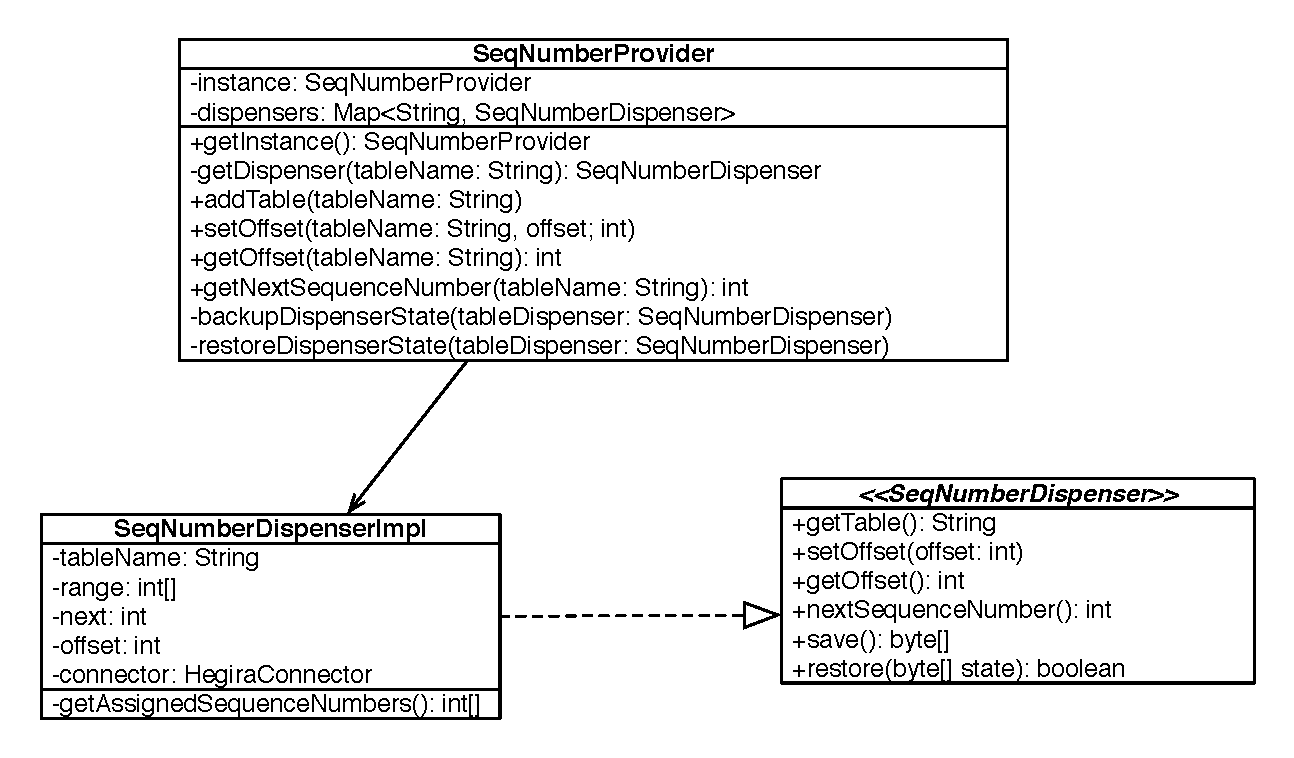
\includegraphics[width=12cm]{images/seq_provider}
  \caption{Sequence numbers handling architecture}
  \label{fig:seq-provider}
\end{figure} 

\noindent The \texttt{SeqNumberProvider} keeps an instance of \texttt{SeqNumberDispenser} for each table that needs to be persisted, and it is responsible of:
\begin{enumerate}
\item providing a unique access point when requesting the next assigned sequence number for a table;
\item initializing or restoring the state of the dispenser for each table.
\end{enumerate}
\noindent The first point is performed through the method \texttt{getNextSequenceNumber(String tableName)} that delegates the operation to the correct \texttt{SeqNumberDispenser} associated to the requested table.
Since \texttt{SeqNumberDispenser} is an interface, the actual implementation is delegated to the \texttt{SeqNumberDispenserImpl} class. This mechanism has been used to be able to create more dispensers with different logic.
\noindent The \texttt{SeqNumberDispenserImpl} class maintains internally the assigned range of identifiers provided by the synchronization system by specifying the first and the last element of the range. The class consumes, one by one, the identifiers in the range and, when the range has been completed, requests the next range. This mechanism is internally handled, in fact the \texttt{SeqNumberProvider} is only required to call the \texttt{getNextSequenceNumber()} method on the dispensers.

\noindent The size of the range of sequence numbers requested to the synchronization system, that is used by the \texttt{SeqNumberDispenser}, has been made configurable at run-time. A default range size can be set using the \textit{migration.xml} file, otherwise, a call to the \texttt{setOffset(String tableName, int offset)} method on the \texttt{SeqNumberProvider}, will change, at-runtime, the size of the range of the \texttt{SeqNumberDispenser} responsible for the specified table.

\newparagraph The second functionality is achieved by requesting the state representation to the \texttt{SeqNumberDispenser}(s) (as a \texttt{byte} array), calling the method \texttt{save()} on the dispensers and, then, saving it to a Blob storage, or to a file, depending on the configuration specified inside the \textit{migration.xml} file (described in Appendix \ref{app:migration}). 
\noindent The restoring phase is performed just after construction; if a backup exists either on file or on the Blob storage, the method \texttt{restore(byte[] state)} is called on the dispensers, giving them their state representation to restore.
In this mechanism, the \texttt{SeqNumberProvider} is completely agnostic with respect to the actual state representation chosen by the \texttt{SeqNumberDispenser}(s). This makes future extensibility more easy and less constrained.

\noindent The list of all the tables to be persisted is retrieved from the \texttt{PersistenceMetadata} previously mentioned for named queries.
 
\subsection{Contacting the synchronization system}
The interaction with the synchronization system has been, until now, only described as a method call. Those calls are made on an external library (\texttt{zkWrapper}) which provides an interface to a ZooKeeper instance, in order to communicate with the synchronization system and to receive the assigned sequence numbers.
Since the ZooKeeper library uses threads to handle communication, it was not possible to use this library for Google App Engine since, the App Engine run-time, does not permit to spawn thread.
The main reasons to communicate with the synchronization system are:
\begin{itemize}
\item the migration state listener, that modifies the \texttt{MigrationManager} state accordingly;
\item the \texttt{SeqNumberDispenser}, that needs to retrieve the sequence number assigned to tables.
\end{itemize} 
\noindent The adopted solution was to modify the \texttt{zkWrapper} library to include an HTTP version that handles the calls not by connecting directly to a zookeeper instance, but contacting a remote server through some defined API, that ultimately interacts with the migration system.

\newparagraph A simple structure has been built to make both the \texttt{MigrationManager} and the \texttt{SeqNumberDispenser}(s) transparent to the type of client that is used to retrieve information from the synchronization system. The architecture is shown in figure \ref{fig:zk-adapter}.

\begin{figure}[tbh]
  \centering
  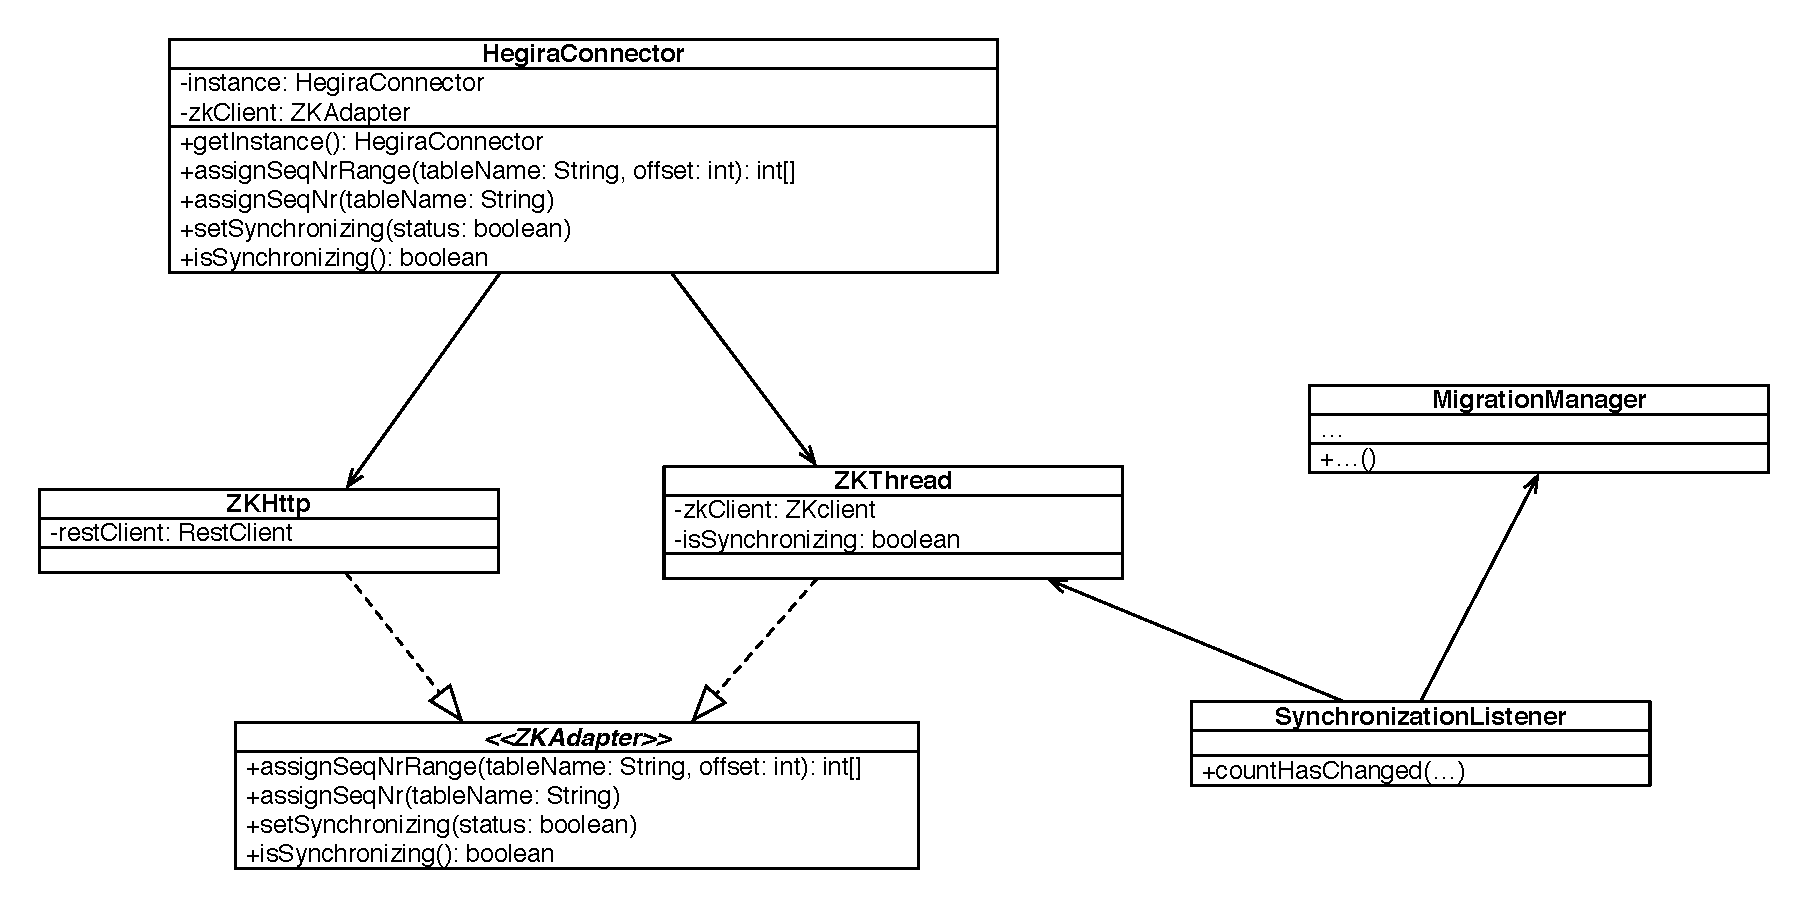
\includegraphics[width=14cm]{images/zk_adapter}
  \caption{Contacting the synchronization system}
  \label{fig:zk-adapter}
\end{figure} 

\noindent The \texttt{HegiraConnector} is the class responsible of deciding which kind of client needs to be instantiated, the decision is done by reading the configuration that the user specified in the \textit{migration.xml} file, which is parsed by the CPIM and kept in the \texttt{CloudMetadata} class. The \texttt{HegiraConnector}  keeps internally an instance of the chosen client and provides access to its method by delegation.
The two available clients implements the interface \texttt{ZKAdapter}, built to uniform the methods of the two implementations.

\paragraph{Thread-based client} If the user deploies the application on a thread-capable cloud environment (for example on IaaS), and configures the \textit{migration.xml} accordingly, an instance of \texttt{ZKThread} is built. This version of the client directly uses the implementation of the library \texttt{zkWrapper} (since there should not be any problem in thread spawning).
The \texttt{isSynchronizing()} method returns a value which is kept inside the \texttt{ZKThread} instance and is queried by the \texttt{MigrationManager}.
Both the state of the \texttt{MigrationManager} and the value inside \texttt{ZKThread} are modified by the \texttt{SynchronizationListener} which is asynchronously notified by the \texttt{zkWrapper} library when the synchronization state changes.

\paragraph{HTTP-based client} In the case in which threads are not supported by the cloud provider (for example on PaaS), the client version that is instantiated (by looking at the configuration) is \texttt{ZKHttp} which uses the API-caller added to the \texttt{zkWrapper} library.
Since no listener can be register to be asynchronously notified of a change in the synchronization state, each call of the \texttt{MigrationManager} to the method \texttt{isSynchronizing()} will perform an API call to the remote server, which will return the state of the synchronization system.

\section{Build statements from user operations}
\label{sec:statements}
In the previous section we have focused on the sequence number retrieval, in this section we will focus on the generation of the Data manipulation queries (DMQs) to be sent to \textit{Hegira} commit-log.

\newparagraph In order to be able to create SQL-like statements both from queries and from objects, the first step has been to introduce the \textit{statement} concept in the CPIM library. This has been done through the abstract class \texttt{Statement} that encapsulate the structure needed for maintaining the necessary data for the statements.
The \texttt{Statement} class is then extended by the three classes: \texttt{InsertStatement}, \texttt{UpdateStatement} and \texttt{DeleteStatement} that basically implement the \texttt{toString()} method to actually build the specific statement.
The class diagram of this statements structure is shown in figure \ref{fig:statements}

\begin{figure}[tbh]
  \centering
  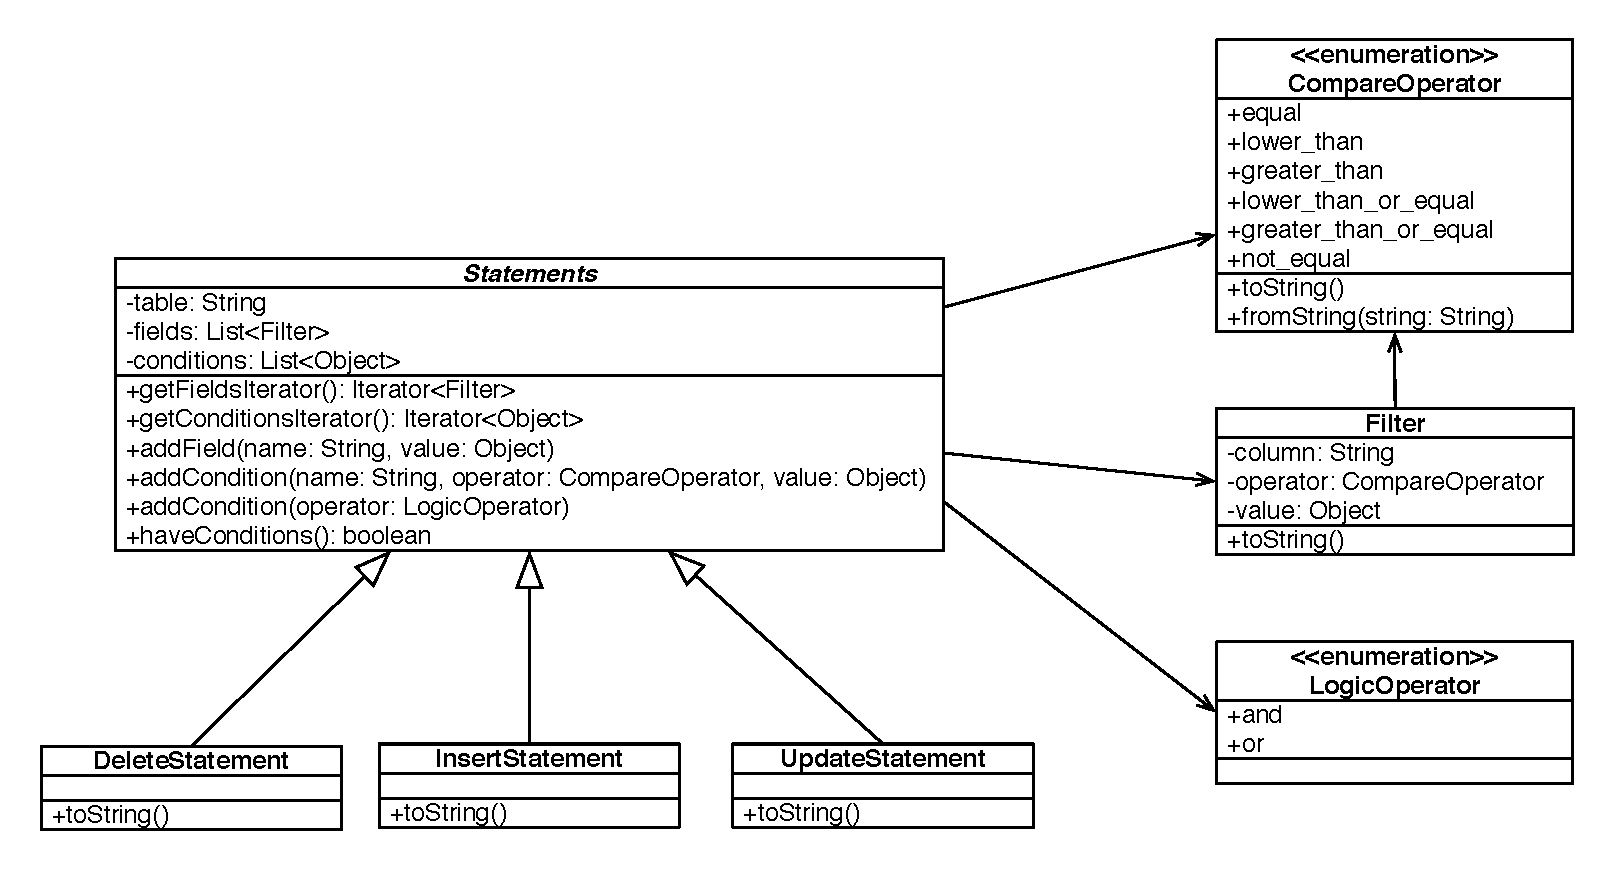
\includegraphics[width=13cm]{images/statements}
  \caption{Statements structure}
  \label{fig:statements}
\end{figure} 

\noindent The \texttt{Statement} class maintains three main fields:
\begin{itemize}
\item \texttt{table}, that contains the table which the statements refer to;
\item \texttt{fields}, that maintains a list of elements that represents, in case of an \textit{UPDATE} statements, the the values inside the \textit{SET} clause and, thus, the column names associated with their value; in case of \textit{INSERT} statements, instead, the column names that should be inserted, and their value;
\item \texttt{conditions}, a linked list of \texttt{Filter} elements and \texttt{CompareOperator} elements, to represents the \textit{WHERE} clause.
\end{itemize} 

\noindent Since not all those elements are needed in all the statements type, specific statements implementations overrides the method that \texttt{Statements} provide for handling those fields to deny their usage. For example since the \textit{INSERT} statement does not permit a \textit{WHERE} clause, trying to add a condition on that kind of statements will result in an \texttt{UnsupportedOperationException}. Another case is the \textit{DELETE} statements that requires only the \textit{WHERE} clause, so when trying to add a \textit{field} the exception is thrown.

\newparagraph After having defined the statements structure, it is then necessary to provide a way to build the correct instance of a statement, starting by the query or by the operation on an object.
To do this in an agile way, a builder class has been implemented.

\begin{figure}[tbh]
  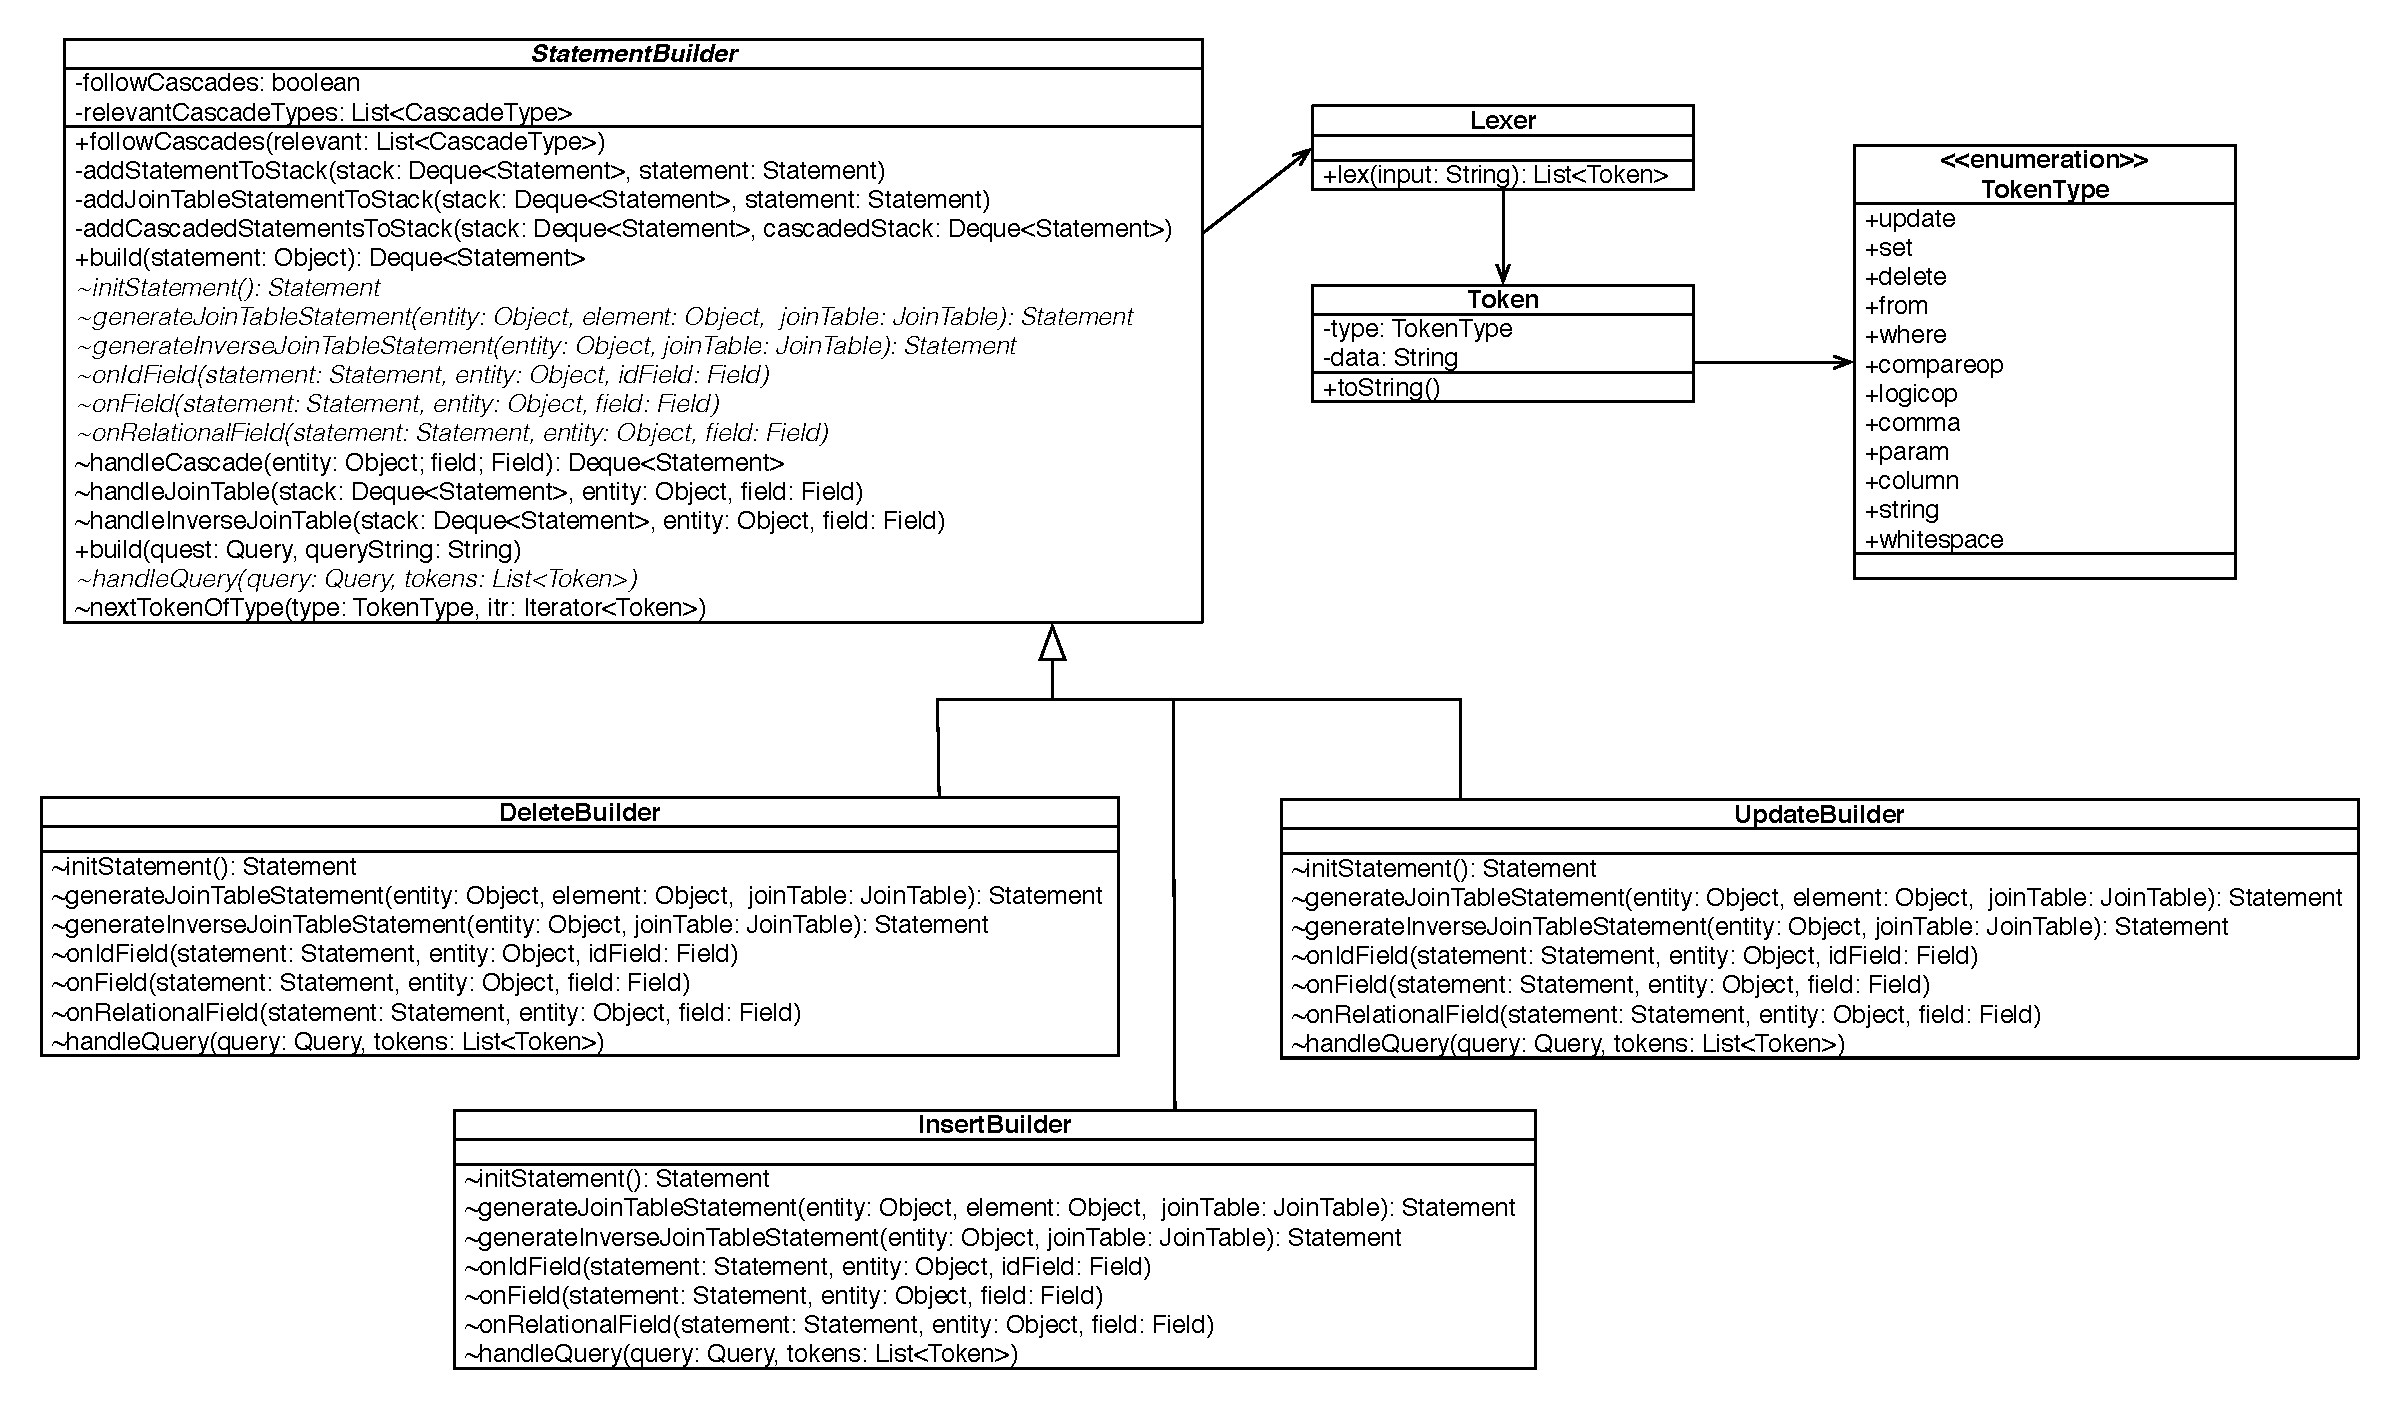
\includegraphics[width=16cm]{images/builders}
  \caption{Statement builders}
  \label{fig:builders}
\end{figure} 

\noindent The class diagram of the builders, shown in figure \ref{fig:builders}, shows that the same pattern used for statements has been adopted.

\noindent The main abstract class \texttt{StatementBuilder} provides the facilities to build a generic statement both from object and from a query string.
Since many operations are the same, for all the three types of statements to be built, the \texttt{StatementBuilder} class provides an implementation of those common behaviors, and it defines some \textit{abstract} methods that are statement-specific and that needs to be implemented in different ways in the three statement builder classes: \texttt{InsertBuilder}, \texttt{UpdateBuilder} and \texttt{DeleteBuilder}.
This degree of abstraction has been possible due to the abstract definition of the \texttt{Statement} class which allows to the \texttt{StatementBuilder} to act independently from the specific statement type and then to delegate to the specific builder in the cases in which such abstraction is not sufficient anymore.

\subsection{Build statements from objects}
The main issue in generating statements from objects are the cascade types. From the JPA specification \cite{book:projpa2}, the user, on relational fields, can define which type of cascade type he wants to be applied upon operations on the entity. The cascade type can be specified through the annotation \texttt{@CascadeType}, four are the relevant values:
\begin{itemize}
\item \texttt{PERSIST}, when the entity is persisted, every related entity is persisted too, without the need of any explicit persist for that entity;
\item \texttt{MERGE}, when the entity is updated, every related entity is updated too, without the need of any explicit merge for that entity;
\item \texttt{REMOVE}, when the entity is deleted, every related entity is deleted too, without the need of any explicit delete for that entity;
\item \texttt{ALL}, which enclose all the previous types.
\end{itemize}

\noindent The problem in supporting such operations is that statements generated by cascade must keep a logical order, an example is reported in the code snippet \ref{code:statements-ordering} in which the insert operation for the \texttt{Employee} should happen after the insert of the \texttt{Department} since the employee maintains a foreign key of the department n which he works.

\begin{lstlisting}[language=SQL, caption=Insert statements ordering example, label=code:statements-ordering]
INSERT INTO Department (id, name) VALUES ('123', 'Computer Science')

INSERT INTO Employee (id, name, department_id) VALUES ('456', 'Fabio', '123')
\end{lstlisting}

\noindent During the development we decided to make the cascade following optional and thus it is configurable in the \textit{migration.xml} file (see the appendix \ref{app:migration} for further details), but also at run-time, by calling the appropriate methods on the class \texttt{BuildersConfiguration}. The statements builders, when created, ask to the \texttt{BuildersConfiguration} class in order to decide if the build process should or should not consider the cascade types and, if its the case they set the \texttt{relevantCascadeTypes} accordingly.
The relevant cascade types have been defined as follow:
\begin{enumerate}
\item \texttt{ALL} and \texttt{PERSIST}, for \textit{INSERT} statements
\item \texttt{ALL} and \texttt{MERGE}, for \textit{UPDATE} statements
\item \texttt{ALL} and \texttt{REMOVE}, for \textit{DELETE} statements
\end{enumerate}
\noindent The statements execution ordering is the same that should be respected for SQL databases in case foreign key constraints are applied, so, for example, \textit{join table statements} must be taken with particular care since inserts in the join table must happen \textbf{after} the insert of the entity itself and deletes in the join table must happen \textbf{before} the delete of the entity itself. An example is reported in the code snippet \ref{code:join-statements}.

\begin{lstlisting}[language=SQL, caption=Join table statements ordering example, label=code:join-statements]
-- insert entities
INSERT INTO Employee (employee_id, name) VALUES ('123', 'Fabio')
INSERT INTO Project (project_id, name) VALUES ('456', 'Apollo')
-- insert record in the join table
INSERT INTO Emp_Proj (id, employee_id, project_id) VALUES ('a', '123', '456')

-- deleting the employee
DELETE FROM Employee_Project WHERE id = 'a'
DELETE FROM Employee WHERE employee_id = '123'
\end{lstlisting}

\newparagraph The abstract builder class \texttt{StatementBuilder} provides a single entry point for statements building, by means of the method \texttt{build(Object entity)}. This method is designed following a template pattern, the designed general algorithm (reported in algorithm \ref{code:statements-building}) performs all the operations needed to build the statement, and it calls several methods defined as abstract, which are implemented in the specific builders (since they require specific logic), and several hook methods that can be overrided by the specific builders to change the algorithm behavior.

\begin{algorithm}[h]
  \scriptsize
  \begin{algorithmic}[1]
  \Function{build}{$object$} 
    \State $stack \gets$ empty queue
    \State $cascadedStack \gets$ empty queue
	\State $statemet \gets$ \Call{initStatement}{}
    \State \Call{setTableName}{$statement$, $object$}
    \ForAll{$field \gets$ \Call{getFields}{$statment$}}
      \If{\Call{isRelational}{$field$} $\And$ \Call{ownRelation}{$field$}}
        \If{$handle$\textunderscore $cascades$}
          \State $cascadedStack \gets$ \Call{handleCascade}{$object$, $field$}
        \EndIf
        \If{\Call{isManyToMany}{$field$}}
          \State \Call{handleJoinTable}{$stack$, $entity$, $field$}
        \Else
        	  \State \Call{onRelationalField}{$statement$, $entity$, $field$}
        	\EndIf
      \Else
        \If{\Call{isManyToMany}{$field$}}
          \State \Call{handleInverseJoinTable}{$stack$, $entity$, $field$}
        	\EndIf
      \EndIf
        \If{\Call{isId}{$field$}}
          \State \Call{onIdField}{$statement$, $entity$, $field$}
        \Else
          \State \Call{onField}{$statement$, $entity$, $field$}
        \EndIf
    \EndFor        
    \State \Call {addStatementToStack}{$stack$, $statement$}
    \If{\Call{isId}{$field$}}
      \State \Call{addCascadedStatementsToStack}{$stack$, $cascadedStack$}
    \EndIf
  \EndFunction
  \end{algorithmic}
  \caption{Template algorithm for statements building}
  \label{code:statements-building}
\end{algorithm}

\noindent Cascade generation is handled through the method \texttt{handleCascade(Object entity, Field field)} where \texttt{field} is the field of the entity that represents the related entity. The \texttt{handleCascade} method checks whenever a statements needs to be generated, based on \texttt{relevantCascadeTypes}, and then it recursively calls \texttt{build(Object entity)} passing as \texttt{entity} the related object. 

\subsection{Build statements from JPQL queries}
The main problem for JPQL queries is parsing. Since JPQL is an object querying language, it makes use of an object identifier on which it uses the dot notation to specify the object properties, furthermore JPQL allows the user to define parameter placeholders (the ones starting with ":") that are filled later through the method \texttt{setParameter(String name, Object value)} of the \texttt{Query} class.

\noindent The translation that should be performed is shown in the code snippet \ref{code:query-translation}.

\begin{lstlisting}[language=SQL, caption=JPQL to SQL translation, label=code:query-translation, numbers=none]
-- JPQL query string
UPDATE Test t SET t.name = :name WHERE t.salary >= :salary

-- SQL version
UPDATE Test SET name = 'Fabio' WHERE salary >= '42'
\end{lstlisting} 

\noindent The mapping among \textit{parameter name} and its \textit{value} is kept in the \texttt{CloudQuery} and \texttt{TypedCloudQuery} classes by intercepting the \texttt{setParameter} method on the query.

\newparagraph To solve the parsing problem, the Kundera code was inspected to understand how JPQL queries are parsed, but it turned out they used a custom quite-complex parser, especially for validation purposes. Even looking online no specific JPQL parser has been found so, since we are not interested in validating queries or build complex logic on them, a simple and less time consuming solution was to write a lexer that through regular expressions tokenizes the JPQL string.

\noindent Even the building of statements from queries follows a template pattern, the \texttt{StatementBuilder} class provides the template method \texttt{build(Query query, String queryString)} that tokenizes the query using the lexer and then calls the abstract method \texttt{handleQuery(query, tokens)} that is implemented in \texttt{DeleteBuilder} and in \texttt{UpdateBuilder} which are responsible of iterating over the tokes to build the correct \texttt{Statement} instance.
The \texttt{build(Query query, String queryString)} calls other various hook methods that can be overrided by the specific builders to change the algorithm behavior.

\subsection{Sending statements to Hegira}
Both the method \texttt{propagate(Query query)} and \texttt{propagate(Object entity, OperationType operation)} fill a statement stack which contains the generated statements in the execution order.

\noindent When iterating over the statement stack, statements are extracted one at a time from the head of the stack (LIFO order). Each of the extracted statement is then sent to \texttt{Hegira}.

%\newparagraph \textbf{TODO update when this part will be done}

\section{Interoperability of stored data}
\label{sec:data-interoperability}
The Kundera client described in chapter \ref{chap:kundera} was developed to be as consistent as possible with the other clients, developed by the Kundera staff, to be more likely accepted by the community and so are not thought to store data to be interpreted also by other clients, and thus are not interoperable.
In an optic of data migration, what we want to achieve is that, data stored within a database, and migrated to another one, are still readable from the application without any changes, besides the new database configuration. 

\noindent The problem for Kundera clients are the relationships. Each database has its own way to define identifier for the persisted entities; for example, in Google Datastore there is the \texttt{Key} with a \textit{Kind} and an \textit{identifier}; for Azure there are the \textit{partition-key} and the \textit{row-key}. These concepts are different, but actually quite similar since both databases are key-value columnar databases. 
A solution to the problem would have been to modify the migration system in order to make it aware of the problem and let it translate the relational columns in the format of the target database; in this way, the relational columns should have been identified in some way to let the system recognize them by adding a pre-defined prefix or a suffix to those columns.
Since this solution requires a good amount of changes in the migration system, other solutions have been explored.
 
\newparagraph Back to the concept of identifier, generally, in columnar databases, columns are grouped in a \textit{column family} and set of columns are identified by a \textit{key}, actually the \textit{key} can span among different \textit{column families}, but that is not the case either in Datastore or Azure Tables.
The pair \textless\textit{column family}, \textit{key}\textgreater{} is sufficient to identify an entity (composed by one or more columns), so a mapping is needed between database-specific terminology to the more general one, this mapping is shown in table \ref{table:mapping}.

\begin{table}[h]
\centering
\vspace{1em}
\renewcommand{\arraystretch}{1.4}
\begin{tabular}{lcc}
\hline
\textbf{General concept} & \textbf{Datastore} & \textbf{Azure Tables}\\ 
\hline\hline
Column Family & Kind & partition-key \\
\hline
Key & key-identifier & row-key \\
\hline
\end{tabular}
\caption{Column family and Key mapping among supported databases.}
\label{table:mapping}
\end{table}

\noindent At this point we needed a common way of persisting relationships as column family, and key in a way that is interoperable among both the client extension.
The proposed solution is to persist a string in the form\texttt{columnFamily\textunderscore key}. This solution has to be preferred with respect to the one that required modification of the migration system since the interoperability is achieved transparently by it.

\subsection{Kundera clients modification}
Since lot of work has already been done on the Kundera clients, the modification to them has been made on a separate branch of the projects named \textit{migration}.

\paragraph{Google Datastore} The Datastore extension has been modified to persist relationships as \texttt{kind\textunderscore key-identifier} instead of the \texttt{Key} instance.
Join tables require particular care; Kundera does not provide the class of the entities involved in the join table, but only the column names and the identifier (the one with the \texttt{@Id} annotation). Queries are possible even if the \textit{Kind} is unknown, since Kundera provides the entity class with the entity identifier as arguments to the find operation.
To be more consistent, and to apply the newly defined identifier pattern (\texttt{kind\textunderscore key-identifier}) even for join tables, a map is maintained in the client and built inspecting Kundera meta-data, to keep track of which entity classes are involved in which many to many relationship.

\paragraph{Azure Tables} The Azure Tables extension has been modified too to reflect the newly defined standard for relationships. In Azure Tables relationships were already being saved as \texttt{partition-key\textunderscore row-key} due to the lack of a class similar to \texttt{Key} for Datastore that encapsulate them. The actual problem here is that user can manually handle the partition-key, but it is not a possibility that can be guaranteed anymore since, if an entity is persisted as \texttt{partition-key\textunderscore row-key}, the \textit{partition-key}, if read by the Datastore extension, will be interpreted as a \textit{Kind}.
Since the \textit{Kind} in Datastore extension is the entity table name, it has been decided to lock the Azure Tables \textit{partition-key} to the table name, so that the user cannot decide on its own, since this will break the interoperability of data.

\noindent The same discussion for the join tables previously made for Datastore , also applies for the Azure Tables extension.

\section{Summary}
In this chapter has been described the CPIM structure and the architecture of the NoSQL service before this work. Then has been described how it was possible to integrate Kundera as unique persistence provider in the NoSQL service together wit the problems encountered in the process.

\noindent From section \ref{sec:hegira} has been described the general interaction we wanted to build to make CPIM and Hegira communicate. Then the architecture and the design choices operated in order to develop such interaction, were introduced and described.
